\subsection{ProteomicsDB: protein-level detection in normal tissues}
\label{sec:proteomicsdb}
Gated antigens were chosen for tumour-restricted RNA expression. We asked
whether mass spectrometry agrees at the protein level. For each study gene we
mapped the UniProt accession to its ProteomicsDB target protein and retrieved
every protein-expression row, then joined the sample table (tissue, species,
disease). A normal-tissue sample was defined before any group comparison as
human, disease-free, and in a fixed whitelist of @NWL@ organ and tissue names.

\paragraph{Calibration gate.} Pre-registered gates PASSED: (G1) @NMAP@ of
@NGENES@ genes mapped to a ProteomicsDB target protein (threshold 180);
(G2) CD19 detected in @CDB@ B-lineage samples (threshold 1); (G3) all four
housekeeping controls detected in at least ten normal tissues (minimum
observed @PCMIN@).
\paragraph{Hypothesis H1 (falsified, reversed).} H1 predicted that gated
proteins are detected in fewer distinct normal tissues than background
(one-sided test).
The opposite holds: median @H1G@ versus @H1B@ normal tissues
(one-sided $p=@H1P@$). Gated genes are also detected in some sample more
often (@DG@/@DGN@ versus @DB@/@DBN@, Fisher $p=@H2P@$).

\paragraph{Control H3.} Background contains proteins that mass spectrometry
rarely sees (immunoglobulin and T-cell receptor segments, olfactory
receptors), so the reversal could be detectability alone.
Restricting to genes detected in at least one sample (declared after H1),
the gated excess remains: median @H3G@ versus @H3B@ normal tissues
(@H3GN@ gated, @H3BN@ background; two-sided $p=@H3P@$).
@VERDICT@

\paragraph{AND-gate antigens.} @ANTIGENBLOCK@

\begin{figure}[t]
\centering
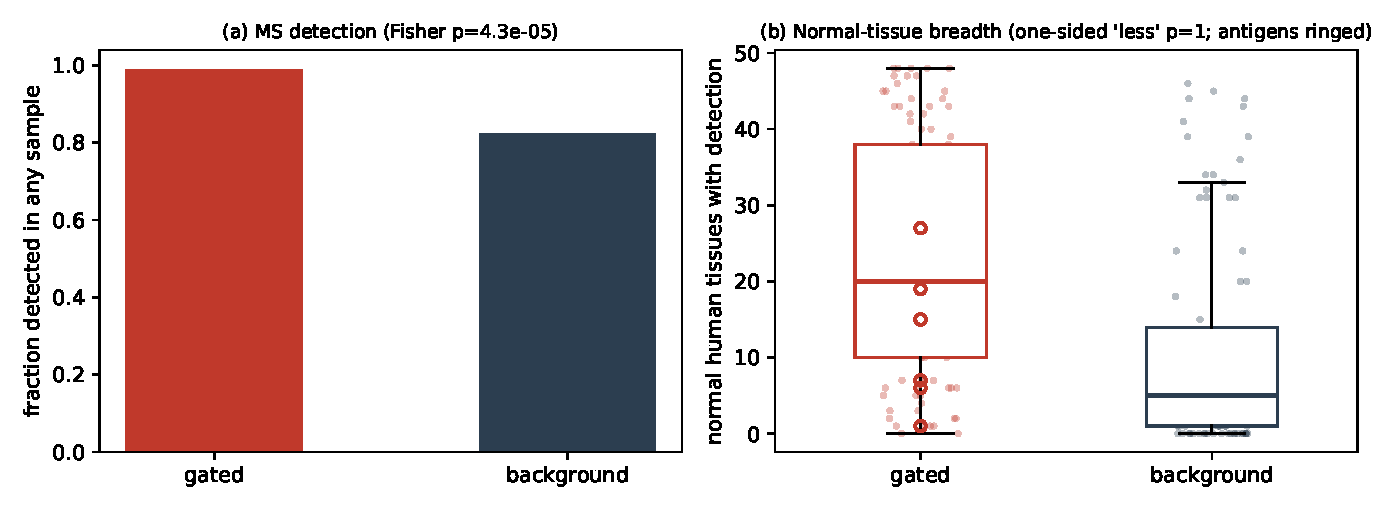
\includegraphics[width=\linewidth]{proteomicsdb_fig.pdf}
\caption{ProteomicsDB protein-level audit. (a) Fraction of mapped genes
detected by mass spectrometry in any sample. (b) Distinct normal human
tissues with detection per gene; AND-gate antigens ringed.}
\label{fig:proteomicsdb}
\end{figure}
